\chapter{DESAIN DAN PERANCANGAN SISTEM}
\label{chapter:desain}

Pada bab ini akan dibahas tentang dasar perancangan sistem yang akan dibuat. Secara khusus akan dibahas mengenai deskripsi umum sistem, perancangan skenario dan arsitektur
sistem.

\section{Deskripsi Umum Sistem}
Tugas akhir ini disusun untuk menangani masalah \textit{monitoring} server dan \textit{computer single-board} dengan menggunakan pola \textit{publish-subscribe}. Pola ini dipilih agar pengguna dapat memilih perangkat mana yang ingin dipantau sehingga tidak semua perangkat terpantau oleh semua orang.

Proses \textit{monitoring} ini diawali dengan pengambilan informasi tiap-tiap server menggunakan SNMP \textit{monitoring tools}. Untuk komputer \textit{single-board} diberikan \textit{agent} untuk mengambil data hasil pemantauan. Kemudian pengguna, atau di sini dapat disebutkan sebagai administrator jaringan, dapat memilih saluran (\textit{subscribe}) \textit{server} atau komputer \textit{single-board} mana yang ingin ia pantau melalui sebuah \textit{agent} yang berupa \textit{web-socket}.

Kemudian, \textit{agent} yang berupa web yang responsif ini akan melanjutkan permintaan ke sebuah \textit{middleware}. \textit{Middleware} yang telah terpola \textit{publish-subscribe} ini akan memproses permintaan tersebut. Kemudian perangkat yang terpilih akan memberikan informasinya (\textit{publish}) melalui \textit{middleware} dan diteruskan kembali ke \textit{agent} berupa notifikasi. Notifikasi ini dapat dilihat oleh admin. Selain itu, \textit{agent} juga mengirimkan notifikasi mengenai keadaan lingkungan dan \textit{server} Pusat Data ITS yang butuh penanganan langsung, seperti \textit{server time out}, suhu ruangan meningkat tajam, ke Telegram. Sehingga administrator bisa langsung bertindak cepat.


\section{Arsitektur Sistem}
Pada subbab ini, dibahas mengenai tahap analisis dan kebutuhan bisnis dan desain dari sistem yang akan dibangun.

\subsection{Desain Umum Sistem}
Sistem \textit{monitoring} perangkat ini merupakan sebuah sistem yang berfungsi sebagai pemantau \textit{server} dan kondisi lingkungan di DPTSI ITS. Sistem ini menggunakan pola \textit{publish-subscribe} dimana pengguna harus berlangganan (\textit{subscribe}) ke suatu perangkat yang memuat data hasil pemantauan. 

Sistem ini terdiri dari 3 (tiga) \textit{server} yaitu \textit{webserver}, \textit{database server}, dan \textit{publish-subscribe server}. Pada \textit{webserver} terdapat aplikasi dan \textit{websocket}. Kemudian terdapat pula REST API yang berfungsi sebagai transaktor data dari \textit{webserver} ke \textit{database server}.

Pengguna yang melakukan fitur selain memantau perangkat akan mengirimkan permintaan (\textit{request}) HTTP ke REST API. REST API kemudian menyalurkan permintaan ke \textit{database server}. Setelah itu REST API akan mengirimkan respon (\textit{response}) ke aplikasi.

Untuk fitur pemantauan server, maka aplikasi akan mengakses \textit{websocket}. \textit{Websocket} ini bertugas untuk mengakses \textit{publish-subscribe server} dimana data yang dihasilkan dari pemantauan oleh Nagios disimpan oleh \textit{publish-subscribe server} ini. Penjelasan dari desain umum arsitektur sistem akan ditampilkan pada Gambar \ref{fig:arsiumum}.

\begin{figure}[H]
	\centering
	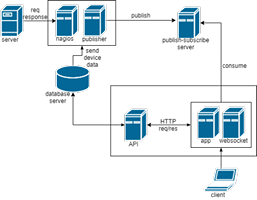
\includegraphics[width=9cm,height=8cm]{assets/images/diagram-arsi.png}
	\caption{Desain Umum Sistem}
	\label{fig:arsiumum}
\end{figure}


\subsection{Desain \textit{Publisher Server}}
Pada \textit{publisher server}, Nagios dipasang untuk memantau keadaan kinerja dari suatu \textit{server}. Kemudian, dipasang pula NRPE untuk mengeksekusi \textit{plugin} Nagios dari jauh. Alasan utama menggunakan NRPE ini adalah memungkinkan Nagios untuk memantau sumber daya "lokal" (seperti beban CPU, penggunaan memori, dan sebagainya). NRPE ini diaplikasikan dengan check-nrpe.

Setiap \textit{server} yang dipantau dimasukkan ke sebuah \textit{thread} baru agar dapat berjalan secara paralel. Kemudian, pada \textit{thread} tersebut setiap \textit{server} terkait akan diperiksa kinerjanya dengan NRPE. Hasil dari pemeriksaan dikirim ke \textit{publish-subscribe server} melalui sebuah \textit{exchange} yang telah diikat dengan sebuah \textit{message queue} yang sudah diinisiasi sebelumnya. Desain dari \textit{publisher server} digambarkan pada Gambar \ref{fig:publisher}

\begin{figure}[H]
	\centering
	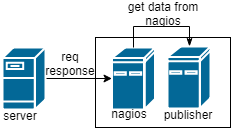
\includegraphics[width=9cm,height=8cm]{assets/images/publisher.png}
	\caption{Desain Publisher Server}
	\label{fig:publisher}
\end{figure}


\subsection{Desain \textit{Publish-Subscribe Server}}
\textit{Publish-subscribe server} adalah sebuah \textit{server} yang berfungsi sebagai wadah untuk menampung pesan dari \textit{publisher} yang mengirimkan data hasil pemantauan oleh Nagios. Pada \textit{server} ini terpasang Rabbitmq sebagai \textit{message broker}. Seluruh pesan yang dikirimkan oleh publisher ditampung ke \textit{publish -subscribe server} melalui sebuah \textit{exchange} yang diikat dengan sebuah \textit{queue}. Setelah itu, \textit{server} akan menyimpan pesan dalam \textit{queue} tersebut hingga ada konsumen, yakni \textit{websocket server}, yang meminta data tersebut untuk dikirimkan.

Secara umum, desain dari \textit{Publish-Subscribe Server} dapat
dilihat pada Gambar \ref{fig:pubsub}.

\begin{figure}[H]
	\centering
	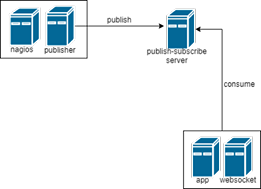
\includegraphics[width=9cm,height=8cm]{assets/images/pubsub.png}
	\caption{Desain Publish-Subscribe Server}
	\label{fig:pubsub}
\end{figure}

\subsection{Desain Webserver}
Pada server ini, terdapat \textit{application server} dan \textit{websocket}. \textit{Websocket} digunakan untuk mengambil data yang dikirimkan oleh \textit{publisher}. Istilahnya, \textit{websocket} ini bertindak sebagai konsumen oleh klien. Data yang diterima sifatnya \textit{realtime} yang berarti merupakan data-data terbaru. 

Konsumen akan membuat sebuah \textit{queue} dengan nama yang ditentukan oleh klien. Nama dari \textit{queue} tersebut ditentukan dengan membuat \textit{string} UUID versi 4 secara acak. Setelah \textit{queue} berhasil dibuat, konsumen membuat \textit{exchange}. Jumlah \textit{exchange} yang terbuat sama banyaknya dengan jumlah \textit{server} yang terdaftar di sistem. Penamaan \textit{exchange} disesuaikan dengan ID masing-masing \textit{server} yang juga berformat UUID versi 4. 

Pembuatan \textit{queue} dan \textit{exchange} ini dilakukan jika \textit{queue} dan \textit{exchange} belum terdaftar pada \textit{publish-subscribe server}. Jika sudah terdaftar, maka tidak dilakukan pembuatan \textit{queue} dan \textit{exchange} lagi. Setelah \textit{queue} dan \textit{exchange} terbuat, maka dilakukan pengikatan (\textit{binding}) \textit{queue} oleh \textit{exchange}. \textit{Queue} dapat diikat oleh satu atau lebih \textit{exchange}. 

Selain itu, semua fitur selain memantau \textit{server} diaplikasikan di \textit{application server}. Fitur-fitur tersebut adalah:
\begin{itemize}
	\item memasukkan data perangkat beserta \textit{service}-nya,
	\item mengubah data perangkat,
	\item menghapus perangkat,
	\item melakukan \textit{subscribe} pada perangkat yang dipilih,
	\item melakukan \textit{unsubscribe}
\end{itemize}


\subsection{Desain \textit{Database Server}}
Desain \textit{database} pada sistem ini adalah seperti yang digambarkan pada Gambar \ref{fig:pdm} di bawah ini. 

\begin{figure}[H]
	\centering
	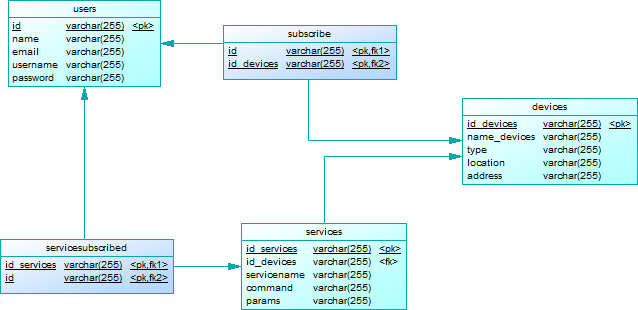
\includegraphics[width=9cm,height=8cm]{assets/images/pdm.png}
	\caption{Physical Data Model}
	\label{fig:pdm}
\end{figure}

Terdapat 5 (lima) tabel pada \textit{database} ini. 3 (tiga) tabel di antaranya adalah tabel berentitas kuat dan merupakan tabel utama pada sistem ini, yaitu: users, devices, dan services. 2 (dua) tabel lainnya merupakan tabel hasil dari relasi \textit{many-to-many}, yaitu tabel subscribe dan servicesubscribe. 

Tabel subscribe ini digunakan untuk menyimpan data pengguna yang melakukan \textit{subscribe} ke suatu \textit{server}. Dan pengguna juga dapat melakukan \textit{subscribe} ke \textit{service} yang dimiliki oleh \textit{server}. \textit{Service} ini berguna untuk mengetahui informasi apa saja yang ada pada tiap perangkat. Tiap \textit{service} memiliki \textit{command} yang berbeda.

\subsection{Desain REST API}
REST API merupakan implementasi dari API (\textit{Application Programming Interface}). REST (\textit{Representional State Transfer}) sendiri adalah suatu arsitektur metode komunikasi yang menggunakan protokol HTTP untuk pertukaran data. Metode ini sering diterapkan dalam pengembangan aplikasi. Tujuan dari REST API yang diterapkan pada pengembangan aplikasi adalah agar sistem memiliki performa yang cepat namun berjalan dengan baik. Sistem juga menjadi mudah dikembangkan terutama dalam hal pertukaran dan komunikasi data. 

URL pada API biasa disebut \textit{endpoint}. Pada sistem ini, terdapat beberapa \textit{endpoint} yang mana masing-masing \textit{endpoint} memiliki \textit{endpoint-endpoint} lagi. 

\textit{Application server} mengirimkan HTTP \textit{request} ke API. Kemudian, API akan melakukan transaksi dengan \textit{database}. Setelah mendapatkan data, maka API akan mengirimkan HTTP \textit{response} ke \textit{application server}. 

Desain dari REST API dapat dilihat pada Gambar \ref{fig:api}. 

\begin{figure}[H]
	\centering
	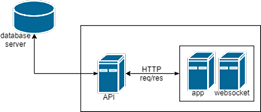
\includegraphics[scale=0.75]{assets/images/rest-api.png}
	\caption{Desain Umum Sistem}
	\label{fig:api}
\end{figure}